\documentclass[../main.tex]{subfiles} % 需要pdf封面

\begin{document}

在本项目中,
按键是关键模块,
我们使用如下代码测试按键响应情况

\lstinputlisting[language=c]{../../src/tests/test_key.c}

该程序每毫秒检测一次按键,
程序内部有按键缓冲,
显示到led灯,
按键缓冲检测按键按下四次,
最右边四个灯同时亮起,
说明按键按下,
并将按下的按键送到数码管显示,

测试结果如\cref{fig:test_key},
测试结果符合预期,
表明按键状态良好。

\begin{figure}[H]
  \centering
    \begin{subfigure}[b]{0.2\textwidth}
    \centering
    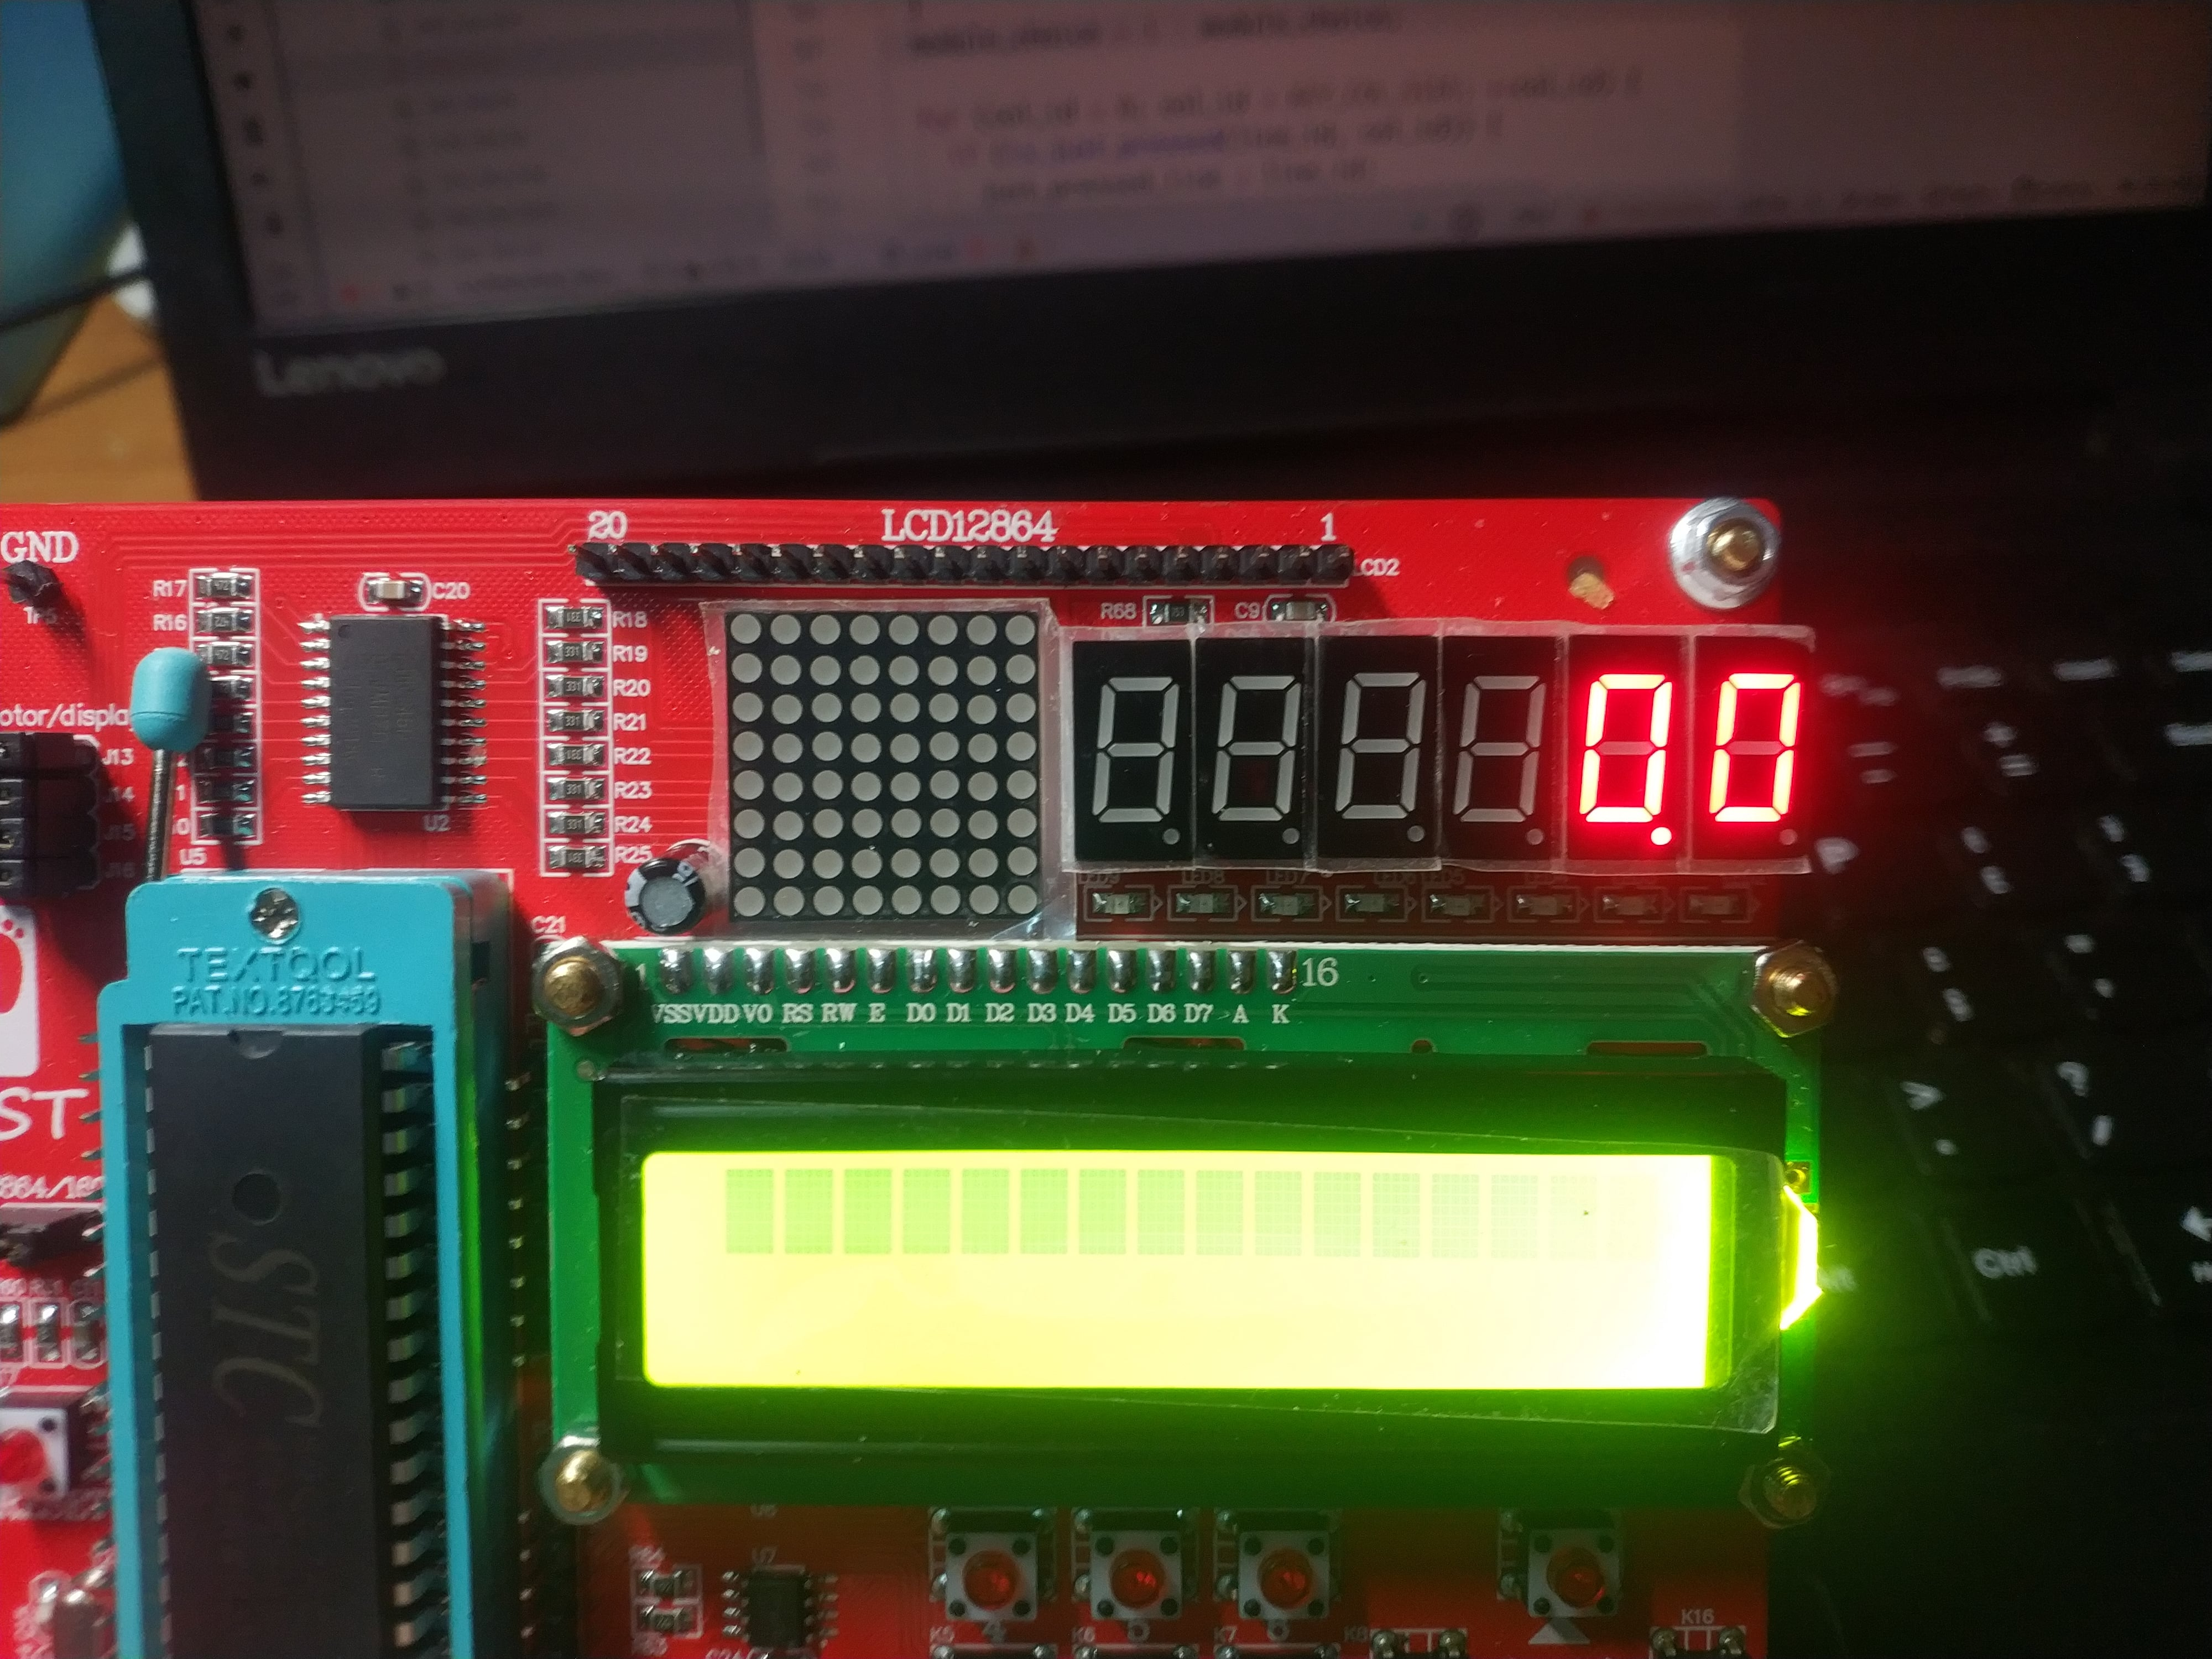
\includegraphics[width=\textwidth]{test_key_1}
    \caption{初始状态没有按键按下,数码管显示0.0}
    \label{fig:test_key_1}
  \end{subfigure}
  \hfill
  \begin{subfigure}[b]{0.2\textwidth}
    \centering
    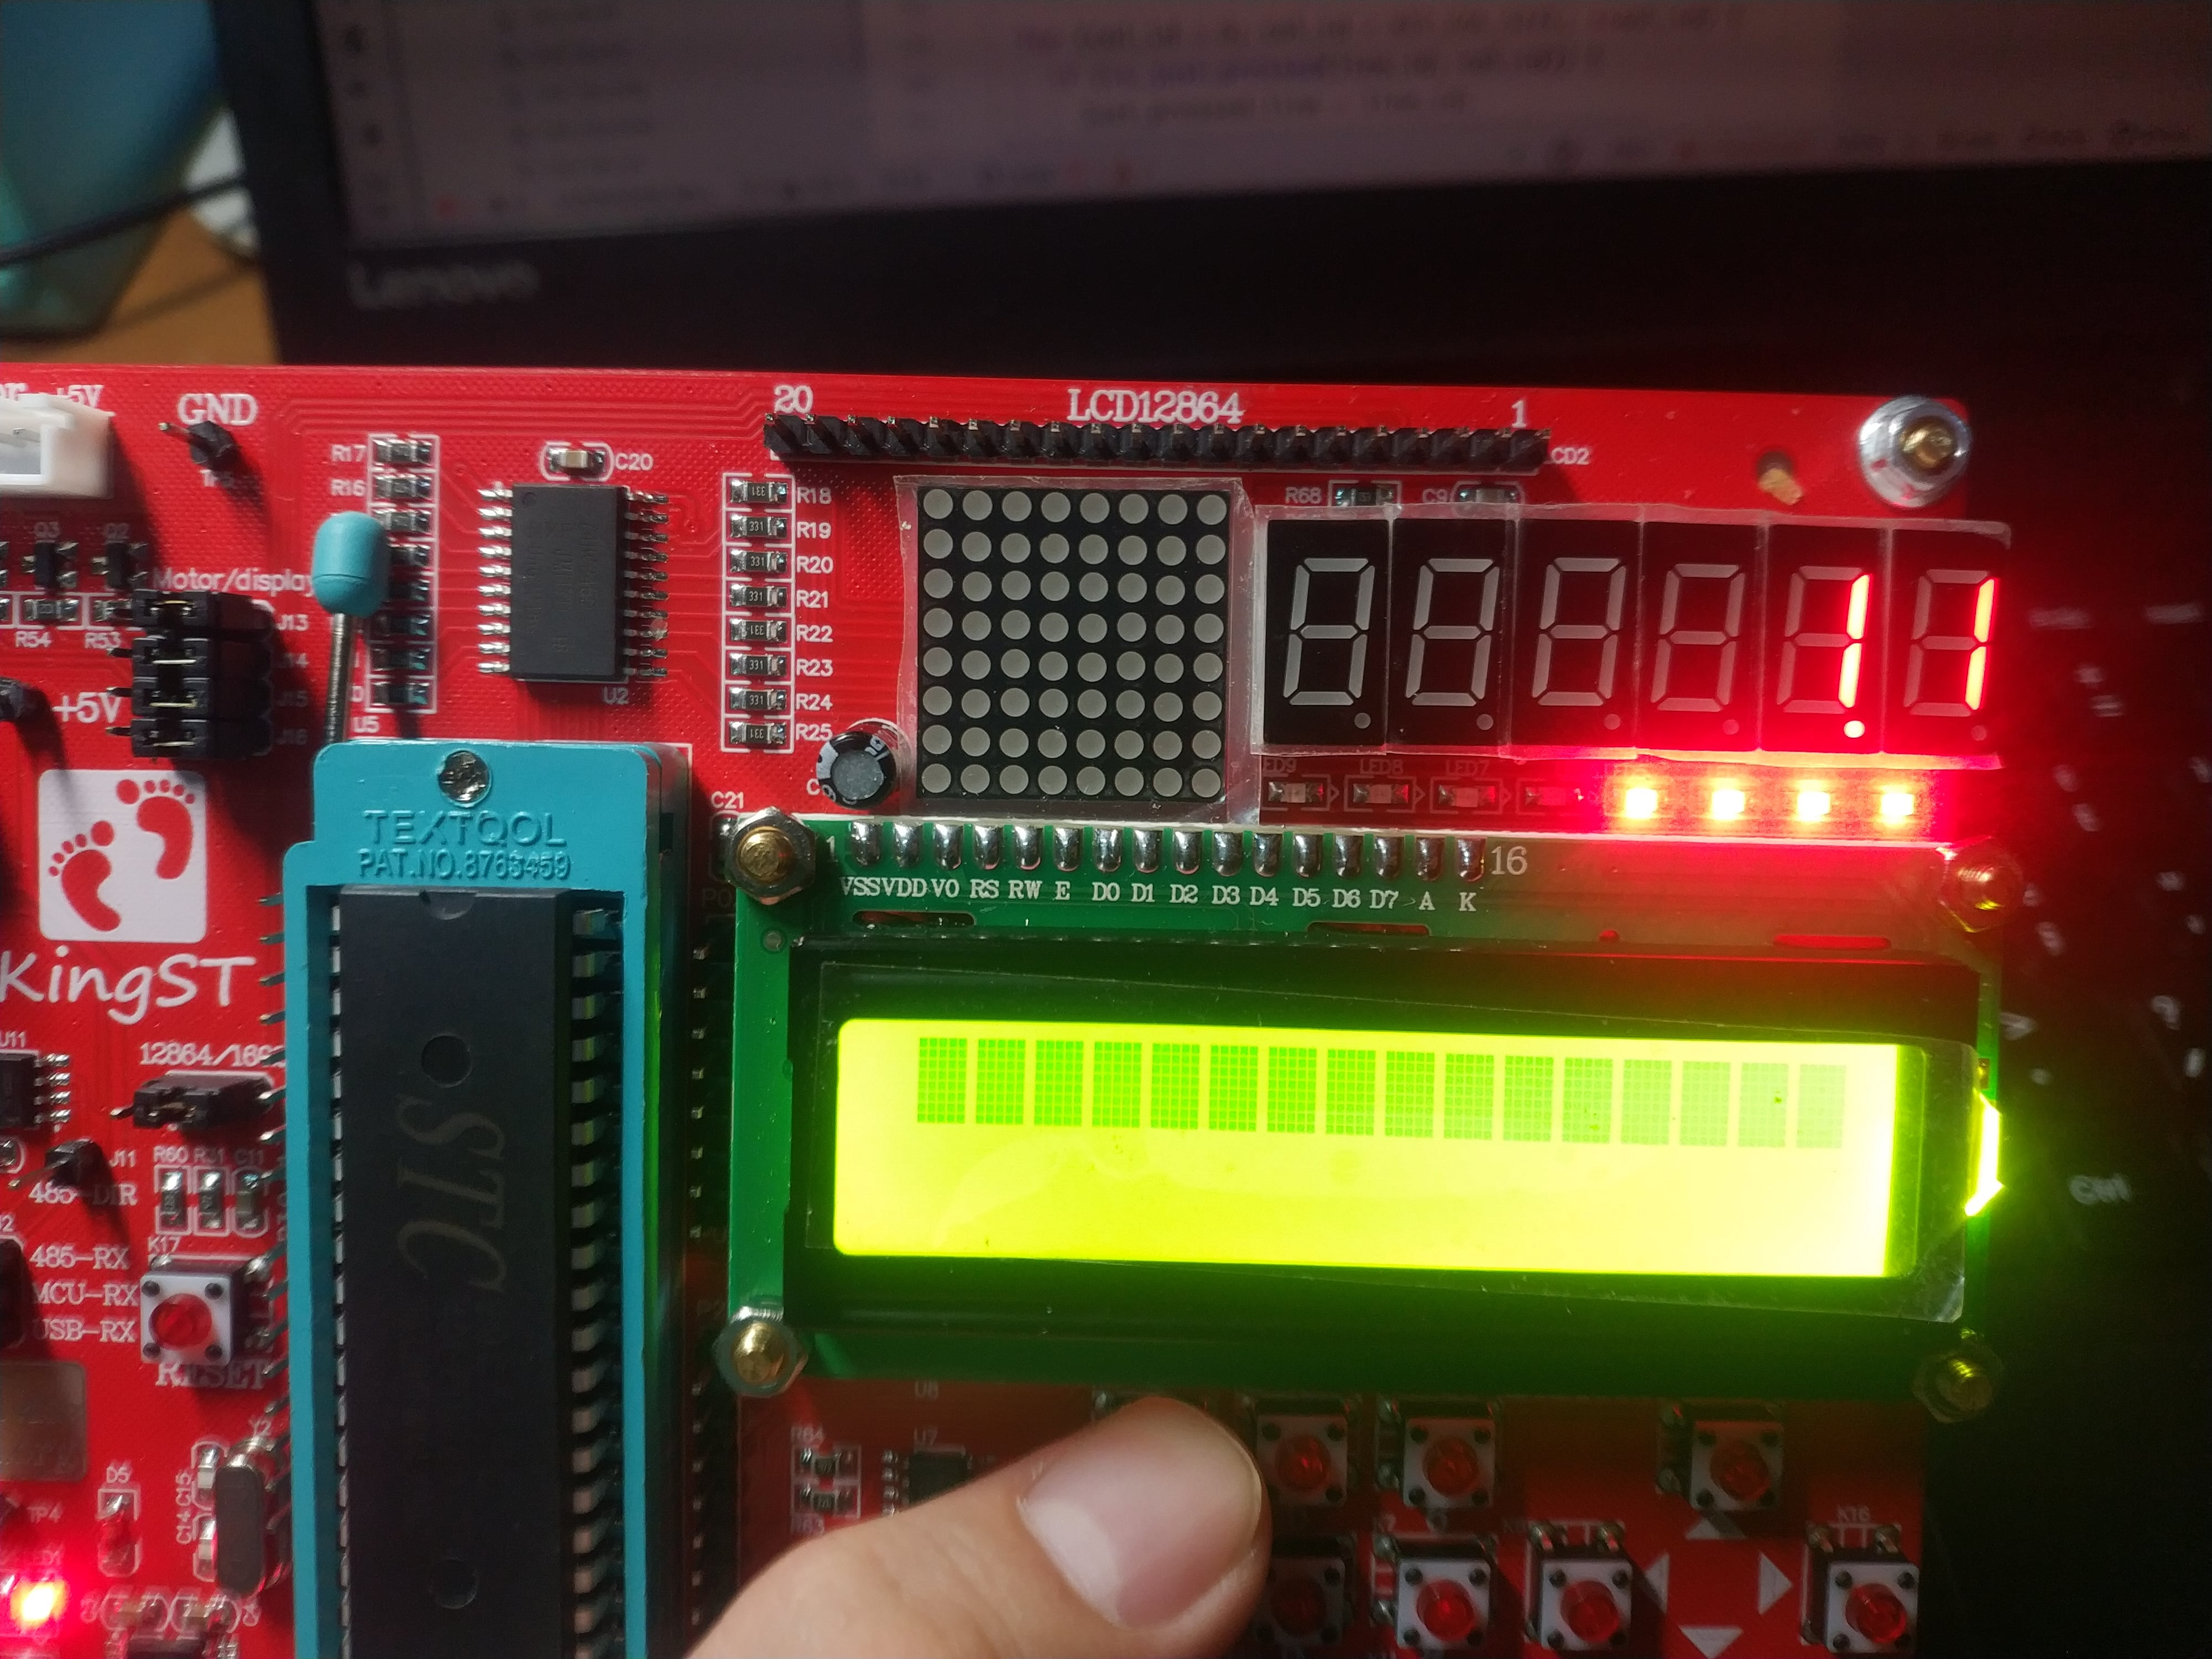
\includegraphics[width=\textwidth]{test_key_2}
    \caption{按下按键$k_{11}$,led灯亮起,
    同时数码管刷新为1.1}
    \label{fig:three sin x}
  \end{subfigure}
  \hfill
  \begin{subfigure}[b]{0.2\textwidth}
    \centering
    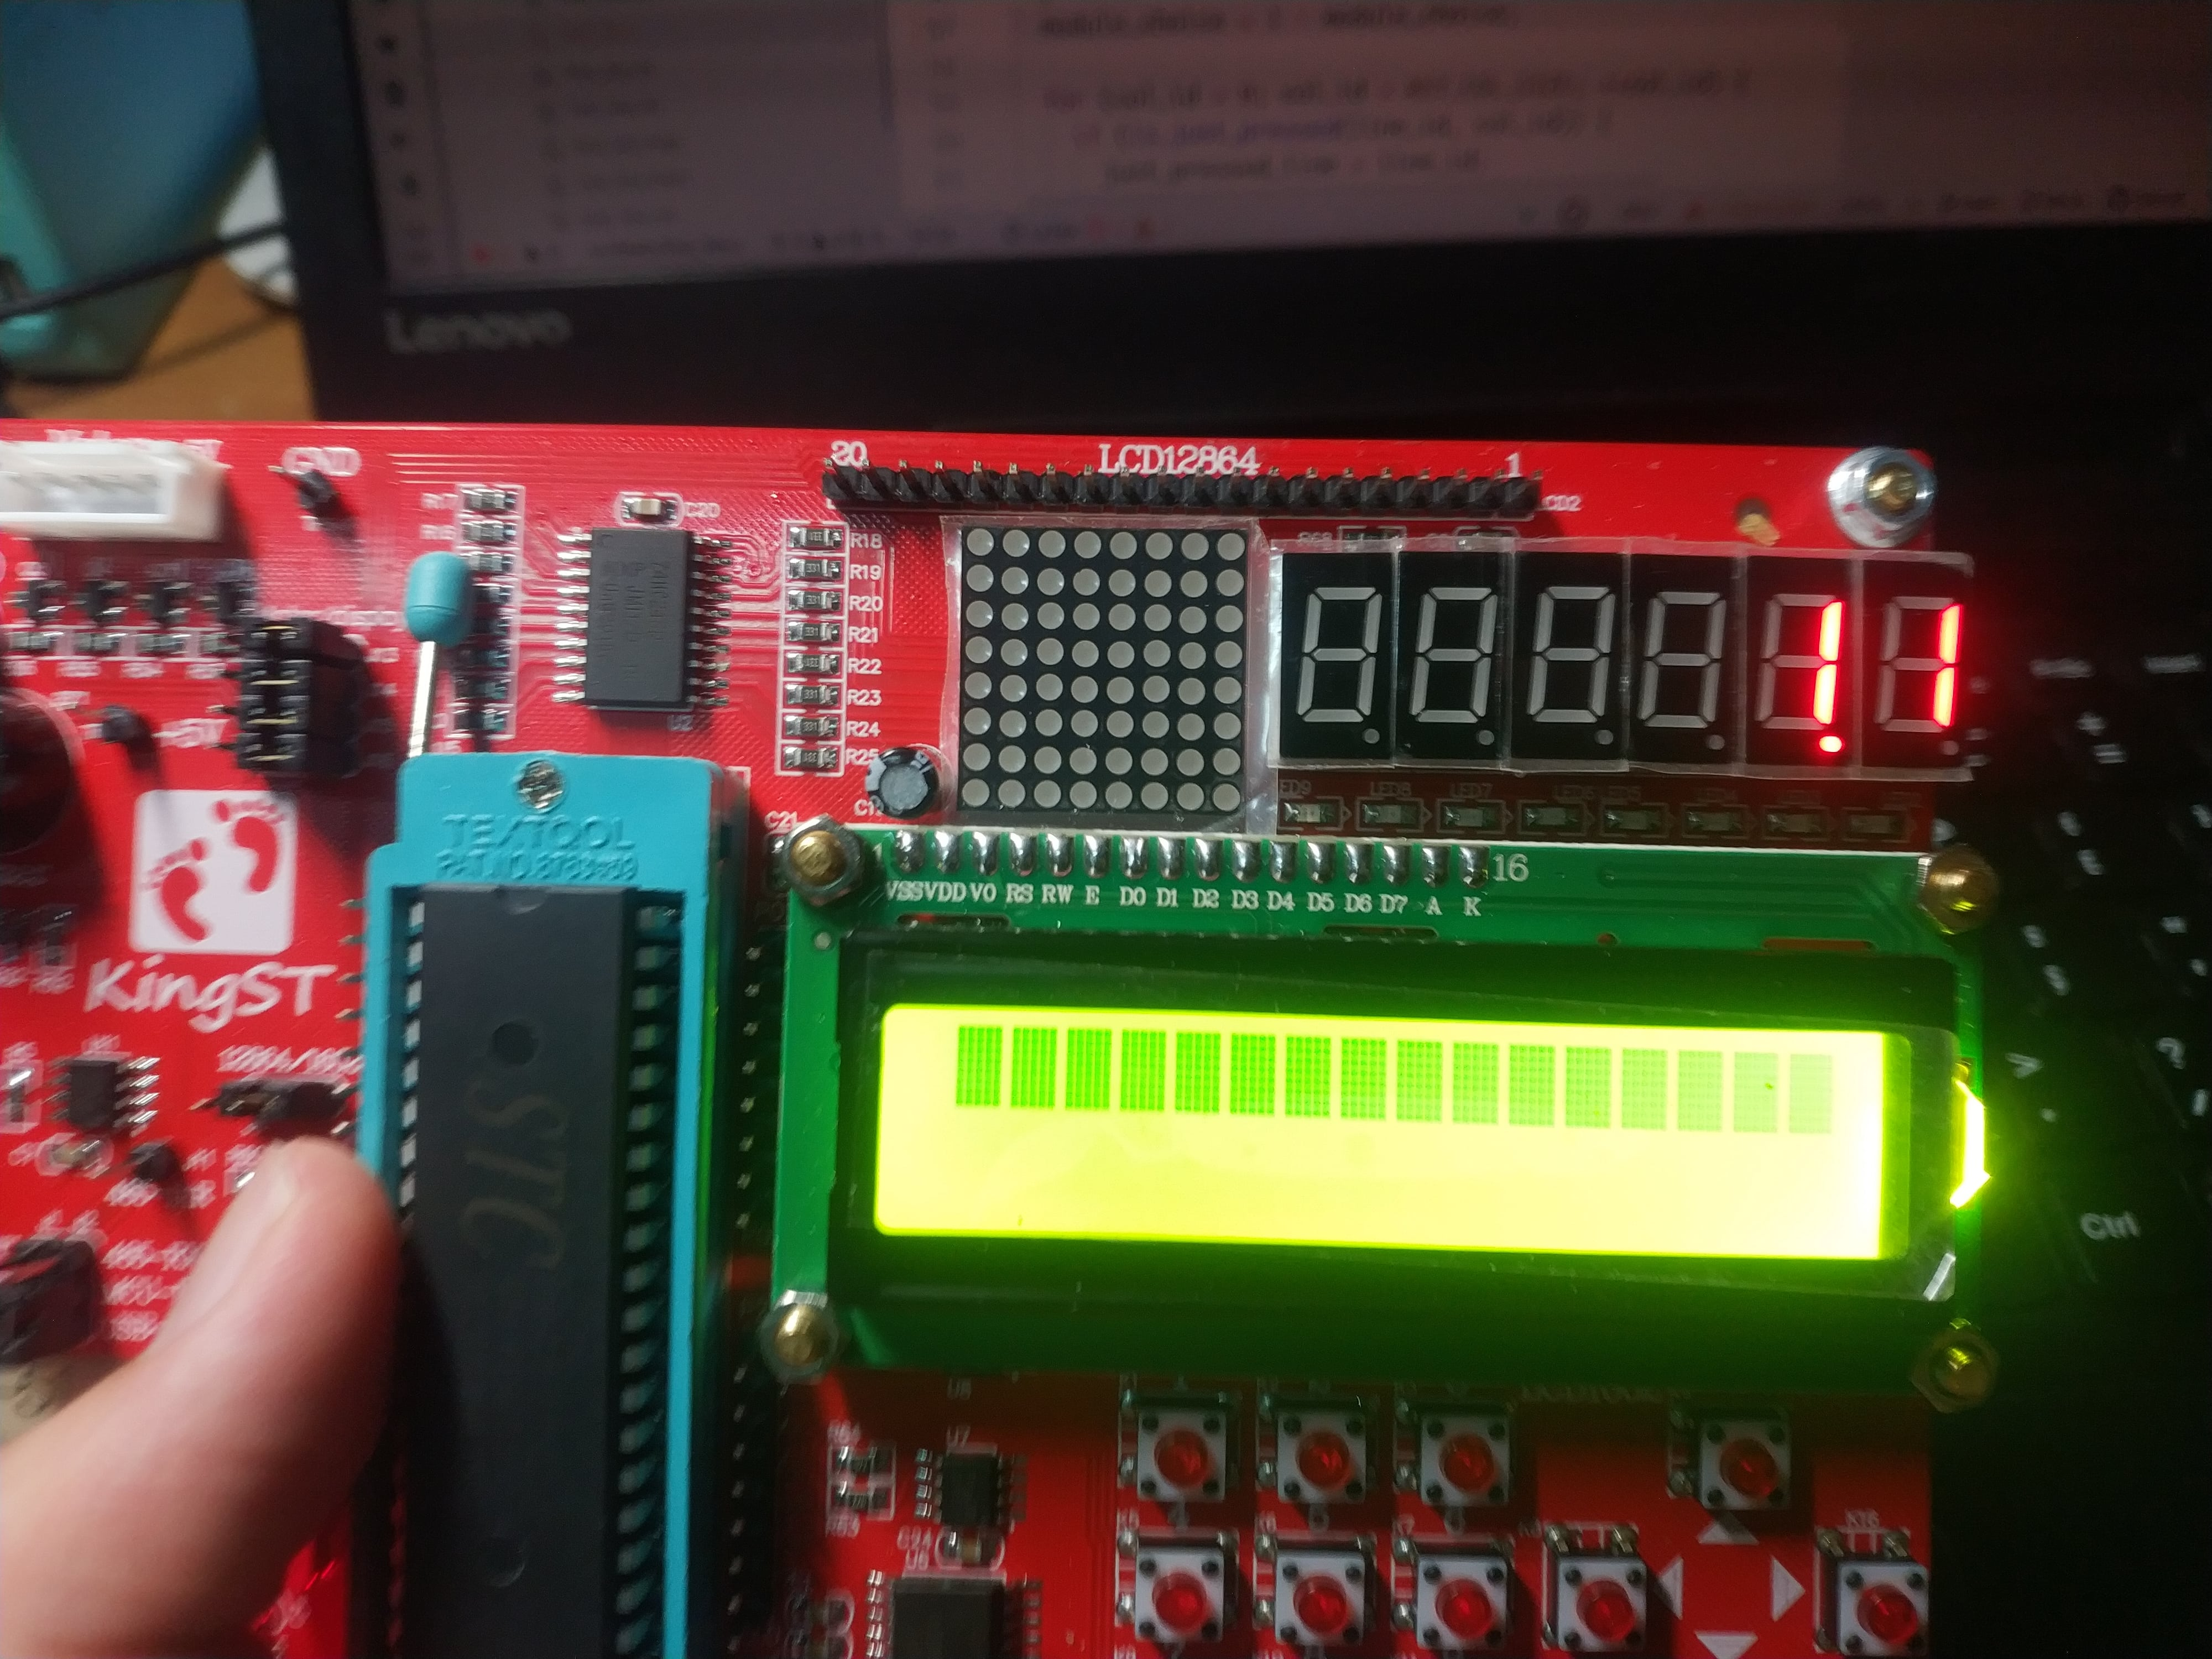
\includegraphics[width=\textwidth]{test_key_3}
    \caption{在没有新的按键按下之前保持该状态,数码管保持不变}
    \label{fig:five over x}
  \end{subfigure}
  \hfill
  \begin{subfigure}[b]{0.2\textwidth}
    \centering
    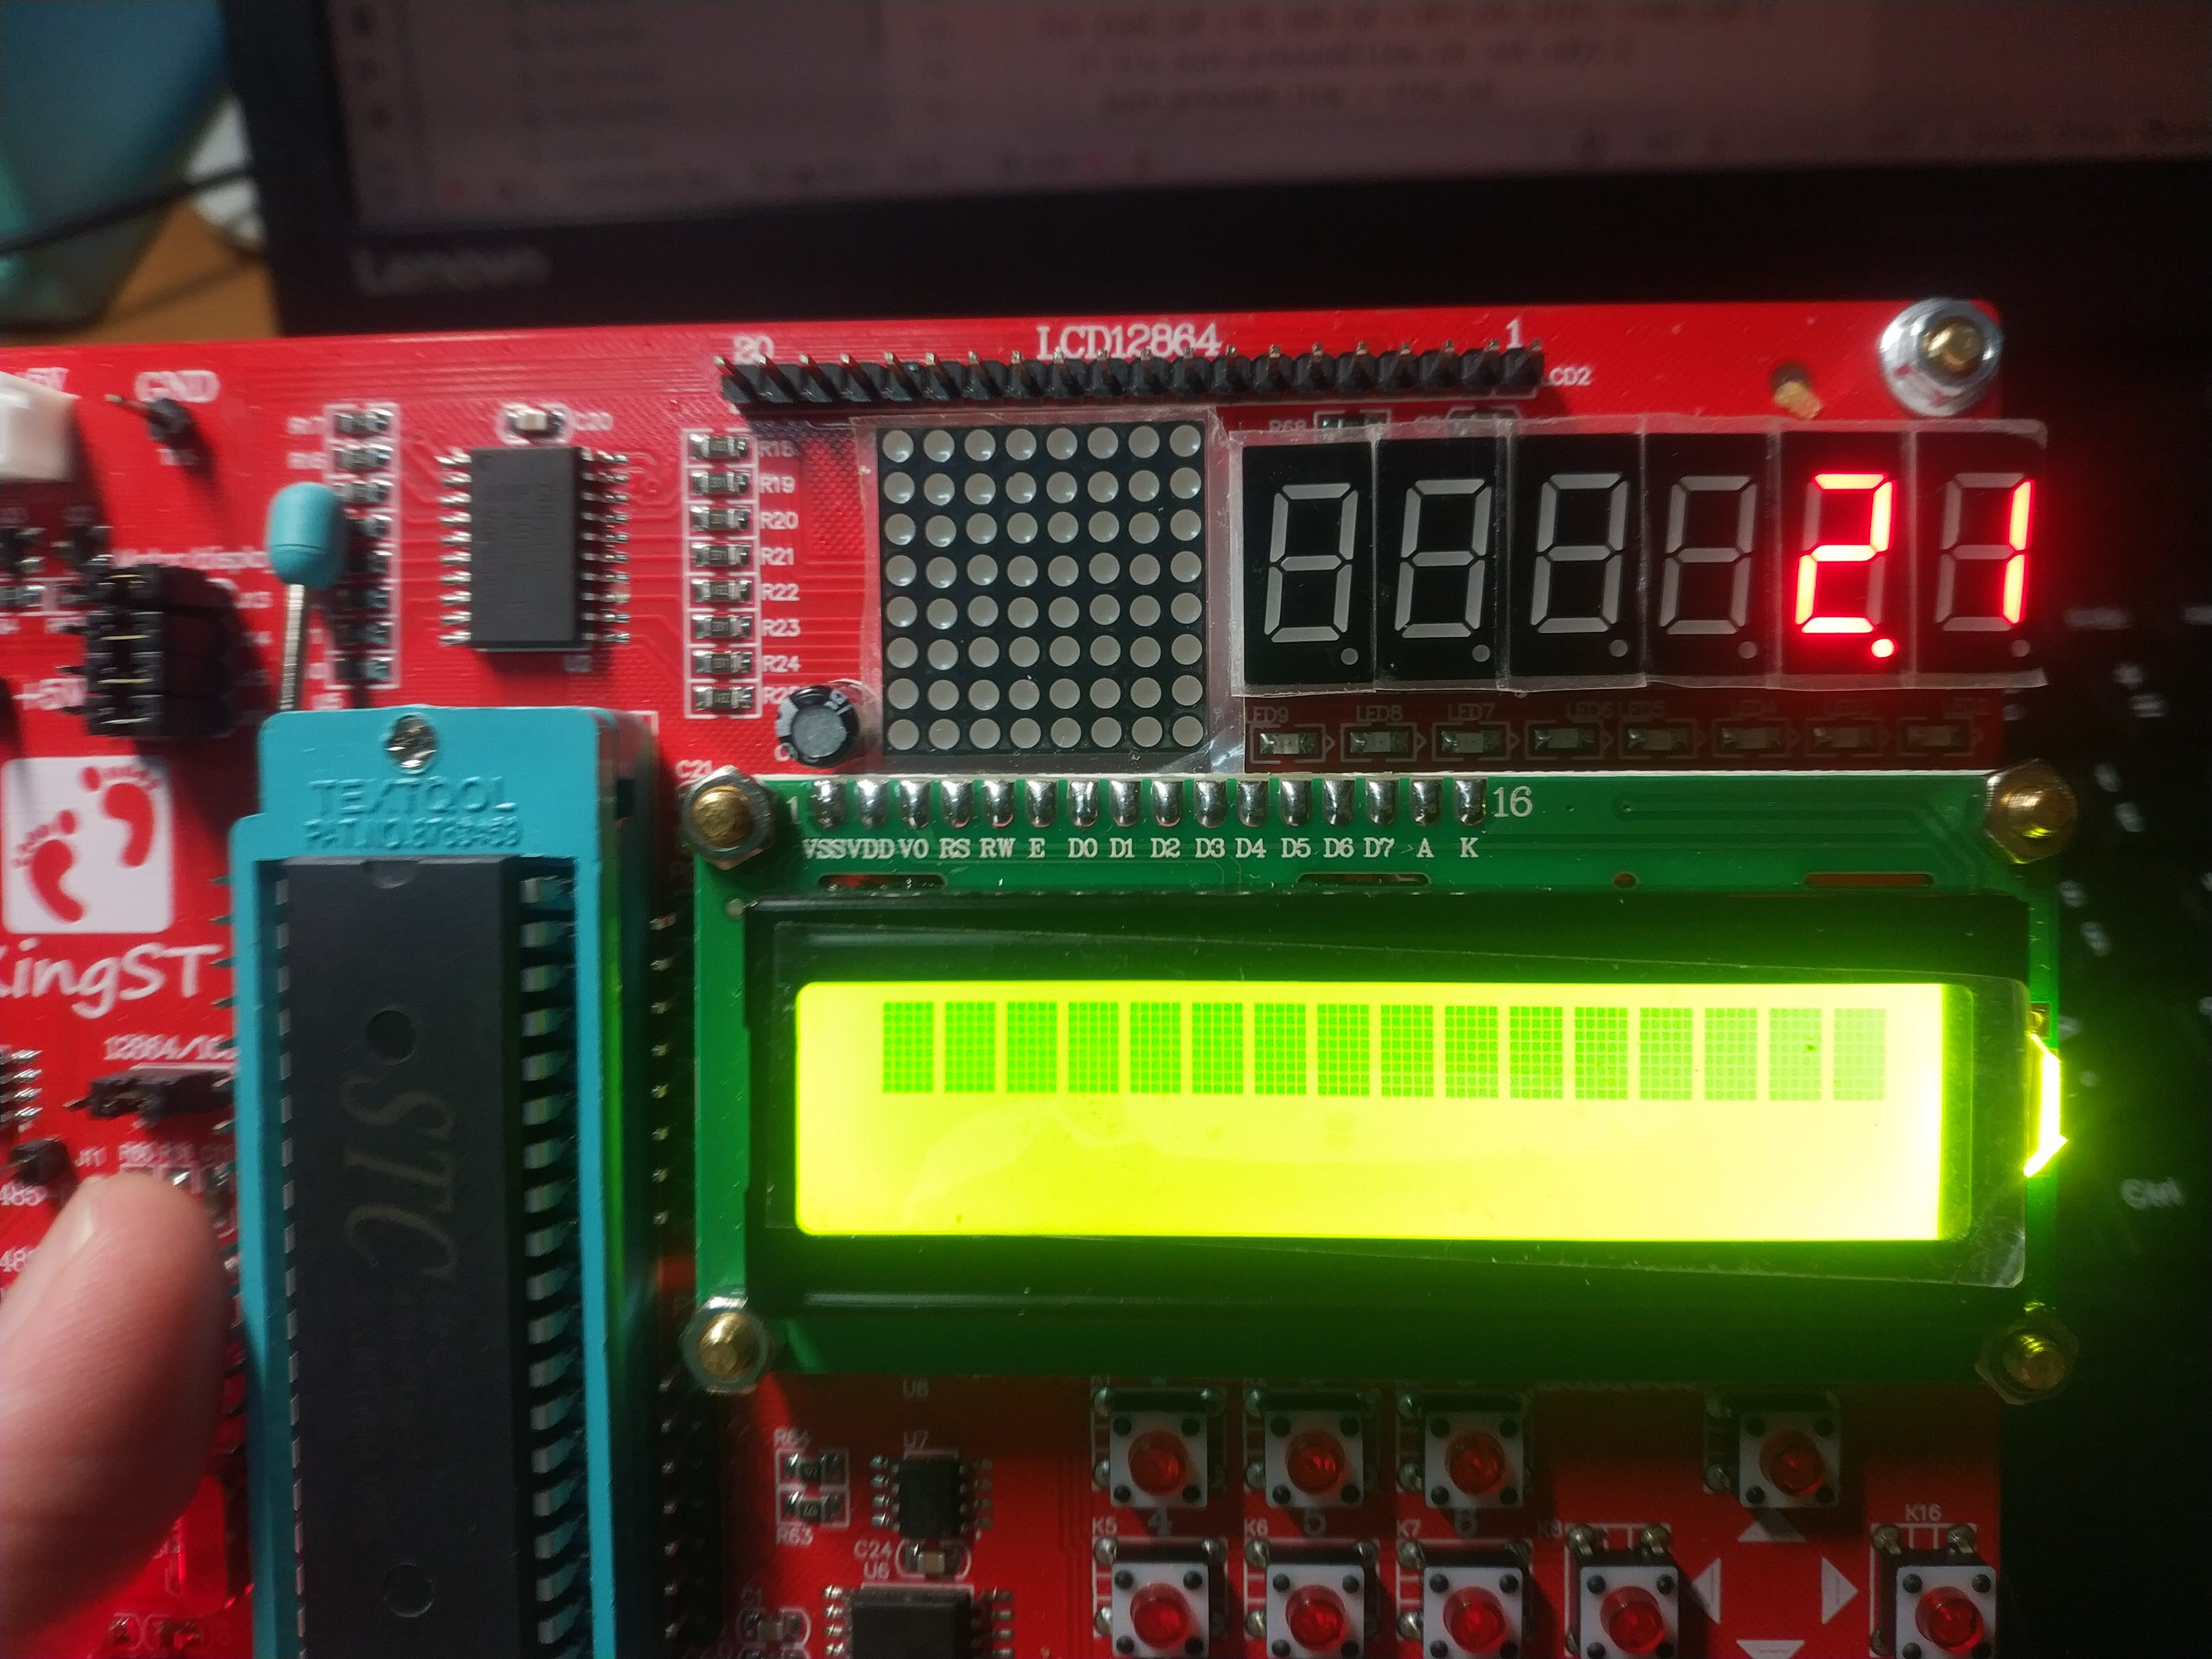
\includegraphics[width=\textwidth]{test_key_4}
    \caption{$k_{21}$按下,数码管刷新为2.2,表明系统检测到该按键}
    \label{fig:five over x}
  \end{subfigure}
  \caption{测试结果}
  \label{fig:test_key}
\end{figure}

\end{document}
